% DOC TYPE E DEF QB SOFTWARE %%%%%%%%%%%%%%%%%%%%%%%%%
\documentclass[12pt]{article}
%%%%%%%%%%%%%%%%%%%% PACKAGES %%%%%%%%%%%%%%%%%%%%
\usepackage[english,italian]{babel}
\usepackage[a4paper, margin=3cm]{geometry}
\usepackage[T1]{fontenc}
\usepackage[utf8]{inputenc}
\usepackage[table]{xcolor}
\usepackage{amsmath}
\usepackage{graphicx}
\usepackage{float}
\usepackage{tabularx}
\usepackage{booktabs}
\usepackage{hyperref}
\usepackage{xcolor}
\usepackage{multicol}
\usepackage{multirow}
\usepackage{soul}
\usepackage{enumitem}
\usepackage{textcomp}
\usepackage{eurosym}
\usepackage{lastpage}
\usepackage{fancyhdr}
\usepackage{adjustbox}
\usepackage{subfiles}

%%%%%%%%%%%%%%%%%%%% COMMAND -> New commands %%%%%%%%%%%%%%%%%%%%
\newcommand{\mailtoQBS}
{
	\href{mailto:qbsoftware.swe@gmail.com}{qbsoftware.swe@gmail.com}
}

\let\oldpar\paragraph
\renewcommand{\paragraph}[1]{\oldpar{#1}\mbox{}\\}

%%%%%%%%%%%%%%%%%%%% COMMAND -> Redefine LaTeX Commands %%%%%%%%%%%%%%%%%%%%
\def\title#1{\gdef\THETITLE{#1}}
\def\date#1{\gdef\THEDATE{#1}}
\def\footname#1{\gdef\THEFOOTNAME{#1}}

\let\oldtexteuro\texteuro
\renewcommand{\texteuro}{\euro}

%%%%%%%%%%%%%%%%%%%% STYLES -> Commands %%%%%%%%%%%%%%%%%%%%
\newcommand{\makefirstpage}
{
	\begin{titlepage}
		
		% Defines a new command for the horizontal lines, change thickness here
		\newcommand{\HRule}{\rule{\linewidth}{0.2mm}} 
		
		\center % Center everything on the page
		
		
		%	Heading Sections
		
		\textsc{\LARGE QB Software}\\[.1cm] 
		
\includegraphics[scale=.15]{imgs/qb-software-logo.png}\\[-.1 cm] 
		
\includegraphics[scale=.025]{imgs/x.png}\\[0.5cm]
		
\includegraphics[scale=.3]{imgs/unipd_logo.png}\\[.5cm]
		\textsc{\Large Università degli studi di Padova}\\[0.5cm] 
		\textsc{\large corso di ingegneria del software }\\[0.5cm]
		\textsc{\large anno accademico 2023/2024 }\\[0.5cm]
		
		
		%	Title section and date section
		
		\ifdefined\THEDATE
		\HRule \\[0.4cm]
		{ \huge{ \bfseries {\THETITLE}} \\ [.5cm]
			\THEDATE}\\[0.4cm] 
		\HRule \\[0.4cm]
		\else
		\HRule \\[0.4cm]
		{ \huge{ \bfseries {\THETITLE}} } \\
		\HRule \\[0.4cm]
		\fi
		%
		\textsc{Contatti:} \mailtoQBS\\[0.3cm]
		
		\vfill 
		
	\end{titlepage}
}

%%%%%%%%%%%%%%%%%%%% ACCESSIBILITY %%%%%%%%%%%%%%%%%%%%
\let\oldhref\href
\renewcommand{\href}[2]{\oldhref{#1}{\textcolor{blue}{\ul{#2}}}}

\hypersetup{
	colorlinks = true,
	linkcolor = cyan,
}

%%%%%%%%%%%%%%%%%%%% STYLES -> Settings %%%%%%%%%%%%%%%%%%%%
% Enable header and footer style
\pagestyle{fancy}
\thispagestyle{empty}
\thispagestyle{fancy}
\pagestyle{fancy}

% Header
\setlength{\topmargin}{-40pt}
\setlength{\headsep}{60pt}
\fancyhf{}
\lhead{QB Software}
\setlength{\headheight}{15pt}
\rhead{
\includegraphics[width=1cm]{imgs/qb-software-logo.png}}

% Footer 
\fancyfoot{}
\fancyfoot[L]{\THEFOOTNAME}
\fancyfoot[R]{Pagina \thepage~di~\pageref{LastPage}}
\futurelet\TMPfootrule\def\footrule{\TMPfootrule}
\setcounter{page}{0}
\pagenumbering{arabic}
\renewcommand{\footrulewidth}{0.3pt}

%%%%%%%%%%%%%%%%%%%% ENVIRONMENT %%%%%%%%%%%%%%%%%%%%
% Remove colorless padding in booktabs
\setlength{\aboverulesep}{0cm}
\setlength{\belowrulesep}{0cm}
\setlength{\extrarowheight}{.75ex}

\newenvironment{todo}{
	\rowcolors{2}{cyan!80!black!30!}{cyan!80!black!20!}
	\begin{tabular}{p{3.48cm}>{\raggedright\arraybackslash}p{4cm}>{\raggedright\arraybackslash}p{6.5cm}}
		\toprule
		\rowcolor{gray!20} \textbf{ID}	& \textbf{Interessato} & \textbf{Task} 
		\\\midrule
	}{
		\bottomrule
	\end{tabular}
}

\newenvironment{changelog}{
	\noindent
	{\Large \textbf{Registro delle modifiche}}
	\noindent
	\begin{table}[h]
		\rowcolors{2}{cyan!80!black!30!}{cyan!80!black!20!}
		\begin{adjustbox}{width=\textwidth}
			\begin{tabular}{|c|c|p{2.35cm}|c|p{3.3cm}|}
				\hline
				\rowcolor{gray!20}
				\textbf{V.} & \textbf{Data} & \textbf{Membro} & \textbf{Ruolo} & \textbf{Descrizione} \\
				
				\hline
			}{
				\hline
			\end{tabular}
		\end{adjustbox}
	\end{table}
	
	\clearpage
}

% 1   2    3        4             5            6            7          
% Ver Data Relatore RuoloRelatore DataVerifica Verificatore Descrizione
\newcommand{\newlog}[7]{
	#1 & #5 & #6 & Verificatore & Controllo qualità \\
	   & #2 & #3 & #4           & #7 \\\hline
}

% INFORMAZIONI DOCUMENTO %%%%%%%%%%%%%%%%%%%%%%%%%
\title{Preventivo dei costi e impegni}
\footname{Preventivo dei costi e impegni}

\begin{document}
	% PRIME PAGINE %%%%%%%%%%%%%%%%%%%%%%%%%
	\makefirstpage
	
	% 1   2    3        4             5            6            7          
% Ver Data Relatore RuoloRelatore DataVerifica Verificatore Descrizione
\begin{changelog}
	\newlog{0.3.0}{15/12/2023}{S. Rovea}{Amministratore}{/12/2023}{}{Correzione ed espansione sezione \ref{sec:management_process}}
	\newlog{0.2.0}{02/12/2023}{S. Destro}{Amministratore}{03/12/2023}{A. Feltrin}{Aggiunta sezione su processi organizzativi, sezione \ref{sec:management_process}}
	\newlog{0.1.0}{22/11/2023}{A. Bustreo}{Amministratore}{22/11/2023}{A. Giurisato}{Aggiunto processo supporto per la documentazione, sezione \ref{sec:documentation}. Aggiunta prefazione, sezione \ref{sec:prefazione}}
\end{changelog}
	\clearpage
	
	\tableofcontents
	\clearpage
	
	% CONTENUTO QUI %%%%%%%%%%%%%%%%%%%%%%%%%
	\noindent Con il presente documento il gruppo QB Software riporta il preventivo per il progetto JMAP: il nuovo protocollo per la posta elettronica, calcolato in base a ruoli e relativi costi.
	
	\section{Impegni orari}
	Per lo svolgimento del progetto sono state previste 651 ore da dividere equamente. Ogni componente del gruppo QB Software si impegna a lavorare al progetto per un totale di 93 ore; tali ore saranno suddivise equamente per ciascun ruolo da assumere durante lo svolgimento del progetto.
	
	\begin{figure}[h]
		\centering
		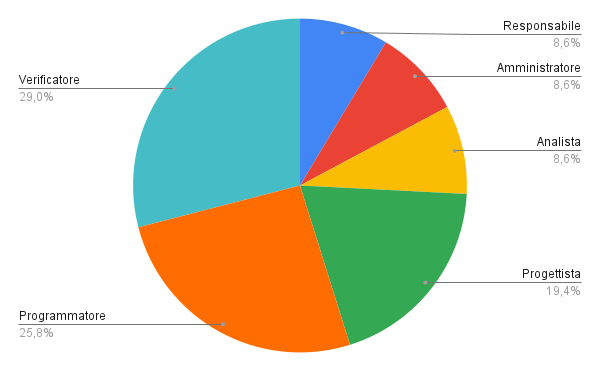
\includegraphics[scale=.6]{imgs/chart.png}
		\caption{grafico indicativo per l'ammontare ore.}
		\label{fig:enter-label}
	\end{figure}
	\clearpage
	
	\section{Considerazione sui ruoli} \label{sec:considerazioni}
	L'ammontare delle ore ripartite come sopra indicato sono frutto di alcune considerazioni che abbiamo fatto:
	
	\subsection{Responsabile e Amministratore}
	Tenendo conto che il responsabile e l'amministratore hanno un ruolo più incentrato sul controllare, coordinare l'operato del gruppo e favorire un buon way of warking collettivo, abbiamo ritenuto che necessitano meno ore produttive rispetto agli altri ruoli per portare a termine i propri compiti.
	
	
	\subsection{Analista}
	Colui che coprirà questo ruolo, dovrà occuparsi di analizzare e studiare i problemi che ostacoleranno l'avanzamento del team. E' fondamentale per avere una buona analisi dei requisiti, tuttavia, non è un ruolo che sarà attivo per l'intera durata del progetto, perciò gli abbiamo assegnato un numero di ore adeguato.
	
	\subsection{Progettista}
	Il progettista si occupa di delle scelte di design e dell'architettura del software, indicando quali sono le soluzioni da implementare per risolvere i problemi evidenziati dagli analisti. Riteniamo che sia un ruolo fondamentale per adempiere in modo corretto ciò che è stato dichiarato nell'analisi dei requisiti, perciò gli abbiamo assegnato un montante ore più elevato rispetto ad altri ruoli.
	
	
	\subsection{Programmatore}
	Il programmatore svolge la funzione di realizzare le scelte implementative fatte dal progettista e  si occupa di una corretta manutenzione del codice nell'intero ciclo di vita del software. Considerando che tale figura sarà  in gran parte presente per tutto lo sviluppo e sarà fondamentale per soddisfare l'analisi dei requisiti, abbiamo deciso di allocare un numero considerevole di ore per svolgere questo ruolo. 
	
	
	\subsection{Verificatore}
	Il verificatore è colui che si assicura che tutte le attività prodotte dai membri del gruppo siano state svolte in maniera consona e corretta, compresa la documentazione. Considerando che sarà ruolo attivo permanentemente, in modo da assicurarci una buona qualità del prodotto, abbiamo deciso di assegnargli il maggior numero di ore.
	
	\section{Preventivo dei costi}
	Il costo finale, basato sulle tariffe orarie dei vari ruoli e l'ammontare ore, è di 12.705,00\texteuro.
	
	\noindent Di seguito una tabella riepilogativa dei costi:
	\newline\newline
	%
	\rowcolors{2}{cyan!80!black!30!}{cyan!80!black!20!}
	\begin{tabularx}{\textwidth}{|X|c|c|c|c|}
		\hline \rowcolor{gray!20}
		\textbf{Ruolo} & \textbf{Ore}         & \textbf{Ore}    & \textbf{Costo}            & \textbf{Costo totale} \\ \rowcolor{gray!20}
		& \textbf{individuali} & \textbf{totali} & \textbf{(\texteuro/ora)}  & \textbf{(\texteuro)}  \\
		\hline\hline
		Responsabile & 8 & 56 & 30 & 1680\\
		\hline
		Amministratore  & 8 & 56 & 20 & 1120\\
		\hline
		Analista & 8 & 56 & 25 & 1400\\
		\hline
		Progettista & 18 & 126 & 25 & 3150\\
		\hline
		Programmatore & 24 & 168 & 15 & 2520\\
		\hline
		Verificatore & 27 & 189 &  15 & 2835\\
		\hline
	\end{tabularx}
	
	\section{Scadenza di consegna}
	Il gruppo stima di consegnare il prodotto finito entro e non oltre il 01/04/2024.
\end{document}